\documentclass[]{scrartcl}
\usepackage{amsmath,amssymb}
%opening
\usepackage{graphicx} 
\begin{document}
\title{CFRM 521 final project\\}
\author{Luke Lee}
\maketitle

\section*{Linear regression} 
Data selection  
\\
To verify that the data chosen for the financial sector(IYF iShare) we fit a linear regression and see if our underlying data can explain the sector returns. As shown in the figure below the selected data have a high $R^2$ value of $81.5 \%$
\begin{figure}[htb]
	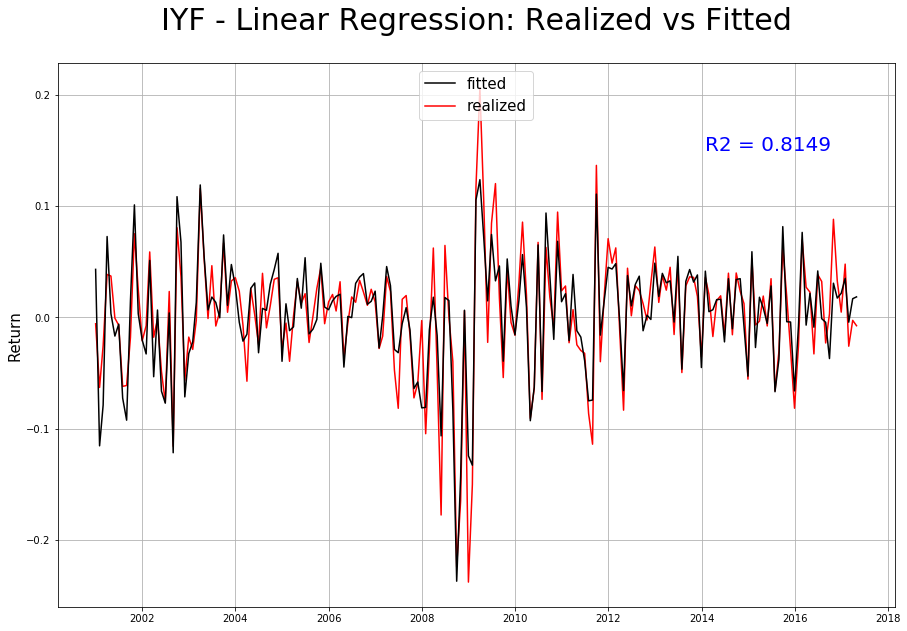
\includegraphics[scale=0.5]{linear_regression_additional_data.png}
\end{figure}
\\
Now that I am satisfied with the data selection, we can move on to testing out more complicated methods that could help us predict this sector out-preforming the benchmark. We calculated our binary predictor variable by taking the excess return of our sector and assigned 1 when it was positive and 0 otherwise.
\\
\section*{Logistic regression}
As mentioned before we are applying a robust method where we use past n years of data to predict certain months ahead and applying this on a rolling basis. In addition to these two parameters, we need to select the penalty type (l1 or l2) and the penalty value($\lambda$). After trying numerous combinations of these parameter's the optimal parameters selected were 5 year looking window, forecasting 3 months ahead, penalty of l2, with lambda of 3.4. 
\begin{figure}[htb]
	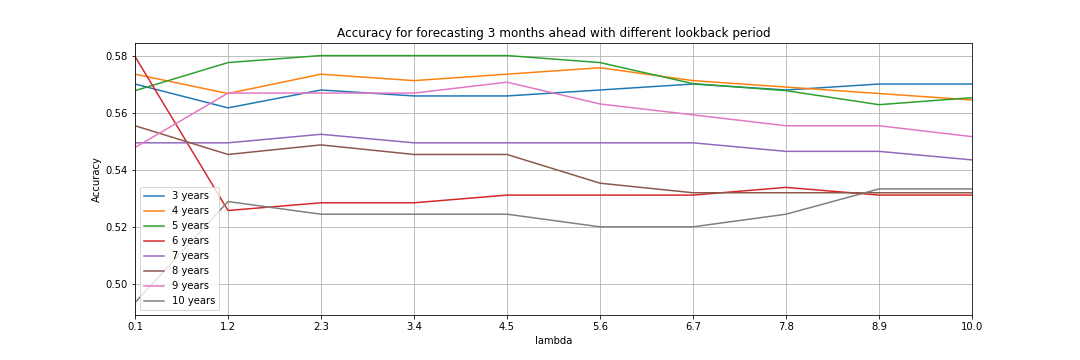
\includegraphics[scale=0.45]{logistic_acf_3month_result.png}
\end{figure}

Here is a comparison of predicted probability against the realized values.
\begin{figure}[htb]
	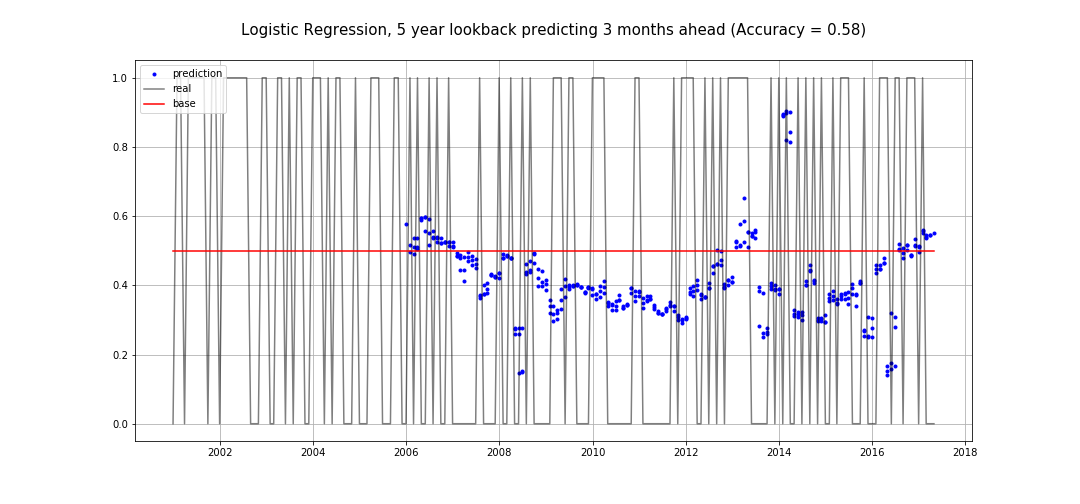
\includegraphics[scale=0.5]{Logistic_regression_5year_3months_result.png}
\end{figure}
The results were not as good as we have hoped for and partly because the probabilities we predict does not seem to be sparse. 

\section*{Elastic Net}
Another method we considered was Elastic Net. Elastic Net's objective function is an extension of linear regression it adds two additional terms, a L1 norm and a L2 norm.
\begin{align*}
\min_{w} \frac{1}{2n}  ||y - Xw||^2_2+\alpha \cdot \text{l1\_ratio} \cdot ||w||_1 + \frac{1}{2} \cdot \alpha \cdot (1 - \text{l1\_ratio}) \cdot ||w||^2_2
\end{align*}

As seen in the objective function, there are two parameters to choose from. $\alpha$ is the penalty parameter and L1\_ratio chooses the ratio of the L1 and L2 penalties.  
  
Unfortunately, the optimal parameter chosen for this model seem to be basically linear regression. The combination with the highest accuracy was when $\alpha$, the penalty parameter, was zero. This simply equates to linear regression.
\begin{figure}[htb]
	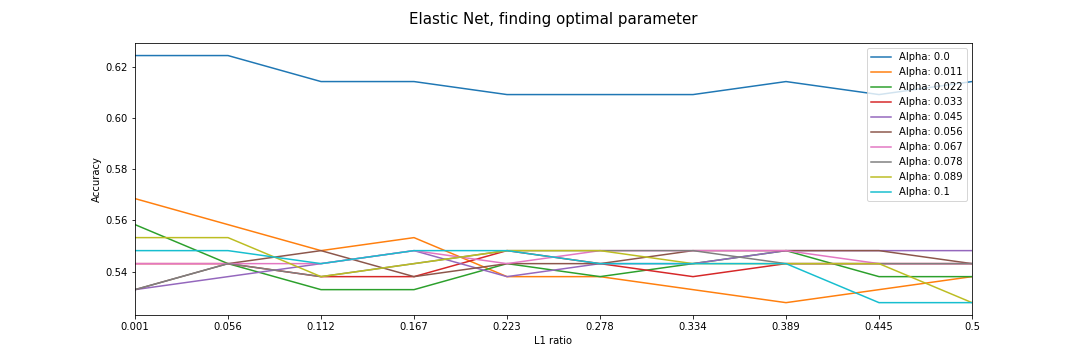
\includegraphics[scale=0.5]{Elastic_regression_cant_beat_linear_reg.png}
\end{figure}

\section*{Back to Linear regression}
Applying the same rolling basis method, linear regression still outperforms the other methods with $70.72\%$ accuracy. Interestingly, linear regression seem to do better with shorter training set data. The optimal parameter for this model was looking back 3 years to predict 3 months return ahead.

\begin{figure}[htb]
	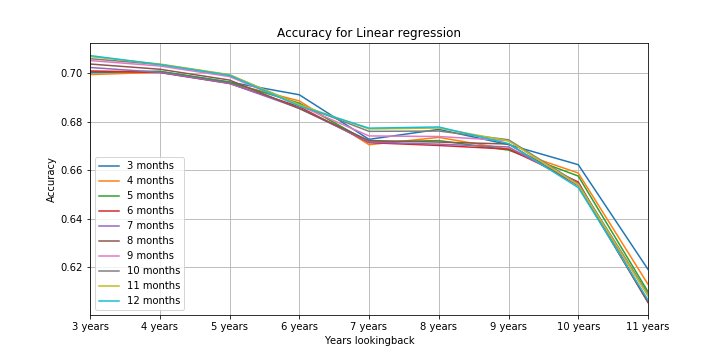
\includegraphics[scale=0.7]{Linear_regression_param.png}
\end{figure}

\end{document}